\newcommand{\rAone}{\mathbf{1}}                          %
\newcommand{\rANeff}{N_C^{\mathrm{eff}}}                 %
\newcommand{\rAgam}{\gamma_C}                            %
\newcommand{\rAVar}{\operatorname{Var}}
\newcommand{\rACov}{\operatorname{Cov}}
\newcommand{\rATm}{\mathcal{T}}                          %
\newcommand{\rAGain}{\mathcal{G}}                        %
\newcommand{\rAHeff}{H_{\mathrm{eff}}}                   %
\newcommand{\rAsh}{\mathrm{sh}}
\newcounter{rAassump}
\renewcommand{\therAassump}{A\arabic{rAassump}}
\newcommand{\rAassume}[1]{\refstepcounter{rAassump}\label{#1}}%
\newtheorem{rAtheorem}{Theorem}[section]
\newtheorem{rAlemma}[rAtheorem]{Lemma}
\newtheorem{rAprop}[rAtheorem]{Proposition}
\newtheorem{rAcor}[rAtheorem]{Corollary}
\newenvironment{rAproof}[1][Proof]{\par\noindent\emph{#1.}\ }{\hfill$\square$\par\medskip}

\section{Setup, conventions and assumptions}\label{rep:setup}

This chapter fixes the physical setting of the whole report.
We define the geometry of a flat homogeneous universe whose spatial sections are three-tori, separate the volume from the shape, and derive the Einstein equations and the minisuperspace action that later chapters use.
We then fix units and conventions, define the two field contents that recur, and state the eight assumptions on which our results rest.
Every later chapter refers to these assumptions by number and does not repeat them.

\subsection{The physical question and the results of this report}
\label{rA:question}

The measured Higgs and top-quark masses place the Standard Model vacuum close to the boundary between stability and metastability~\cite{Degrassi:2012ry,Buttazzo:2013uya,Bednyakov:2015sca,Andreassen:2017rzq}.
Run to high energies, the Higgs quartic coupling $\lambda$ turns negative far below the Planck scale and stays small and negative up to it, so the electroweak vacuum is metastable, with a lifetime much longer than the age of the universe~\cite{Andreassen:2017rzq}.
Whether the vacuum survives the early universe is a separate question.
During inflation the Higgs field fluctuates and feels the spacetime curvature through its non-minimal coupling $\xiH$~\cite{Espinosa:2007qp,Herranen:2014cua,Kearney:2015vba,Espinosa:2015qea,Joti:2017fwe,Markkanen:2018pdo}.
For a minimally coupled plateau inflaton survival requires $\xiH\gtrsim0.06$ at the electroweak scale~\cite{Mantziris:2020rzh}, and $\xiH\gtrsim0.1$ in $R^2$ gravity~\cite{Mantziris:2022fuu}. %
After inflation the oscillating curvature limits $\xiH$ to values below about one~\cite{Herranen:2015ima}. %
All of these bounds concern a universe that is already large and inflating.

A universe that begins small poses the question in a different form.
A contracting flat universe can turn into an expanding one only if its total energy becomes non-positive at the turning point and its stress becomes negative enough to make $\dot H$ positive (Sec.~\ref{rep:trace}).
Classical fields that violate the null energy condition by that much tend to carry ghost or gradient instabilities~\cite{Dubovsky:2005xd,Kobayashi:2016xpl}, and avoiding them takes carefully engineered higher-derivative theories~\cite{Ijjas:2016tpn}.
Quantum fields offer a source without new classical degrees of freedom: on a compact flat space the vacuum energy of untwisted massless bosons is negative and grows as $L^{-4}$ when the space shrinks~\cite{DeWitt:1979dd}.
With a positive vacuum energy this Casimir energy turns a contracting three-torus around along an exact, regular solution, found by Zel'dovich and Starobinsky~\cite{Zeldovich:1984vk} and written in closed form by Guth and Vilenkin~\cite{Guth:2025dal}.
Toroidal universes that begin small were also discussed in Refs.~\cite{Coule:1999wg,Linde:2004nz,Fornal:2026qfq}.
For the Standard Model the turning point is a few thousand Planck lengths across (Sec.~\ref{rep:turning}), and there the quartic coupling is negative.

Does a beginning at such a turning point destroy the electroweak vacuum?
On a small torus the relevant degree of freedom is the Higgs zero mode, the spatially constant mode of the Higgs field, and two effects compete.
A small compact volume catalyzes false-vacuum decay, which then proceeds through a uniform tunneling mode~\cite{Hassan:2026cmp}, as does the Schwinger effect in compact directions~\cite{Brown:2015kgj}.
A small torus also gives the gauge fields zero modes of their own; at this size their zero-point fluctuations are not a small correction, and they couple to the Higgs zero mode through the covariant derivative (Sec.~\ref{rep:zeromodes}).
The Higgs chapters of this report (Secs.~\ref{rep:h-matching}--\ref{rep:h-universality}) show that the second effect prevails down to a finite-volume threshold, and that the threshold turns the question into a criterion on the top-quark mass.

The ingredients have been studied separately.
The Casimir energy of Standard Model fields on circles and tori was computed for compactifications to lower dimensions~\cite{Arkani-Hamed:2007ryu,Fornal:2011tw}, where the violation of the null energy condition by the Casimir energy is what allows the lower-dimensional vacua with horizons to exist~\cite{Arkani-Hamed:2007ryu}.
Fornal recently proposed that our universe originated from an empty, Planck-size three-torus with periodic boundary conditions, whose positive Casimir energy drives its expansion~\cite{Fornal:2026qfq}; that scenario has no turning point and does not treat the Higgs zero mode.
Hamada and Shiu treated Wilson lines together with the high-scale Higgs vacuum in compactifications of the Standard Model on a circle and a two-torus~\cite{Hamada:2017yji}.
The constant modes of gauge fields on a small torus are the leading order of the small-volume expansion of Yang--Mills theory~\cite{Luscher:1982uv,Luscher:1982ma,Luscher:1983gm,Weisz:1986vu,vanBaal:1988va,vanBaal:2000zc}.
Constant gauge fields have been studied classically in Bianchi~I cosmologies~\cite{Darian:1996jf,Jin:2004vh}, and constant abelian backgrounds on tori acquire one-loop masses~\cite{Kirsten:1993ty,Kirsten:1993qp}.
Finite-volume tunneling between degenerate vacua can itself violate the null energy condition and produce a bounce~\cite{Alexandre:2019ygz,Ai:2024dwi}.

The trace anomaly is the second quantum ingredient of a turning point.
The trace of the stress tensor of conformal fields is fixed by the curvature in every state~\cite{Duff:1993wm}.
Anomaly-driven isotropic cosmologies~\cite{Starobinsky:1980te,Fischetti:1979ue} and the damping of anisotropy by quantum effects~\cite{Hu:1978zd,Hartle:1979uf,Hartle:1980nn} are classic.
In the quantum creation of a closed universe studied by Barvinsky and Kamenshchik, the conformal anomaly and the Casimir energy of conformal fields select the instantons and bound the cosmological constant~\cite{Barvinsky:2006uh}; that universe is isotropic and spatially closed, whereas the torus here is flat, carries the Standard Model in the AAA structure, and faces the anisotropic obstruction of Sec.~\ref{rep:trace} and the emptiness gate of Sec.~\ref{rep:gate}.
Mithani and Vilenkin wrote the Friedmann equation of a flat, isotropic Casimir torus with the trace anomaly~\cite{Mithani:2014toa}.
In their oscillating universe, with a negative cosmological constant, the negative Casimir energy balances matter with $w=-2/3$ at the inner turning point, and excited radiation lowers the Casimir coefficient; their torus has periodic fermions, a fixed cubic shape and no Higgs field.
Earlier Casimir bounces used the stress of a single scalar, in a closed static universe~\cite{Herdeiro:2005zj} or in a fluid model of a flat torus~\cite{Godlowski:2007gx}.
The usual turning-point conditions~\cite{Solomons:2001ef} do not tell whether a conformal state can turn an anisotropic universe around; Sec.~\ref{rep:trace} answers this.

A Casimir turning point also leaves something behind.
The shape of a torus is unstable under Casimir back-reaction in two dimensions and in de~Sitter space~\cite{Seriu:1995hc,Ponton:2001hq,COMPACT:2026vdj}, and the shape is the part of the geometry that can survive to the present.
If the fundamental domain is smaller than the last-scattering sphere, the cosmic microwave background (CMB) shows matched circles~\cite{Cornish:1997ab}.
Their absence requires the shortest translation of a three-torus to exceed $0.985$ times the last-scattering diameter $\dLSS\simeq27.7$\,Gpc~\cite{Vaudrevange:2012da,COMPACT:2022nsu}, and Planck likelihood searches give comparable limits~\cite{Planck:2015gmu,COMPACT:2026uzi}. %
A torus somewhat larger than the last-scattering sphere still imprints correlations that are detectable in principle~\cite{COMPACT:2023rkp,Himeno:2026lgh}.
Directional null energy controls the completeness of anisotropic flat cosmologies and bounds their net change of shape, the fossil anisotropy~\cite{Zhou:2026szo}; a Casimir turning point is a concrete quantum source for that fossil.

\paragraph{Results derived in Part~I.}
Our main result concerns the Higgs zero mode (Secs.~\ref{rep:h-matching}--\ref{rep:h-universality}).
At the turning point the zero-point fluctuations of the $W$, $Z$ and hypercharge zero modes confine the Higgs zero mode, so a negative quartic coupling is tolerated down to a finite-volume threshold.
For $\lambda<0$ the Higgs zero mode is a resonance rather than a bound state, and the probability $\Pone$ that it survives the turn along one branch falls steeply as $\lambda$ decreases.
The threshold $\lamc$ is the value of $\lambda(\mub)$ at which $\Pone=1/2$, where $\mub=1/\Lb\simeq3.4\times10^{15}$\,GeV is the matching scale set by the size of the torus at the turn. %
Numerically $\lamc=-0.0121$, with $-0.0091$ and $-0.0152$ for $\Pone=0.9$ and $0.1$. %
The Standard Model value, $\lambda(\mub)=-0.0098$ for the measured masses, lies above it. %
A finite threshold exists in every sector that turns around and keeps a Higgs zero mode among those analysed (the fully periodic torus with an SU(3) center holonomy is not), and its size depends only logarithmically on the duration of the turn (Sec.~\ref{rep:h-universality}).
The scaling law of Sec.~\ref{rep:h-universality} gives $\lamc\approx-0.01$ wherever the gauge zero modes confine the Higgs zero mode; for the spin structures PPA and PAA, which also turn around and keep the zero mode, indicative estimates shift the critical mass by $+0.08$ and $+0.02$\,GeV, and their exact thresholds need an anisotropic model. %

The steep dependence of $\lambda(\mub)$ on the top-quark pole mass $\mt$, $d\lambda(\mub)/d\mt\simeq-0.0066\,{\rm GeV}^{-1}$, comes from the same top-Yukawa running that sets the absolute-stability bound~\cite{Degrassi:2012ry,Buttazzo:2013uya,Bednyakov:2015sca}. %
It converts the threshold into a criterion (Sec.~\ref{rep:h-smmap}): $\Pone>1/2$ if and only if $\mt<172.96$\,GeV, or $\mtbar<163.16$\,GeV for the $\MSbar$ mass $\mtbar\equiv\mtbar(\mtbar)$, at $\alpha_s(M_Z)=0.1180$. %
The Standard Model theory error of this bound is $\pm0.10$\,GeV for $\mt$ and $\pm0.07$\,GeV for $\mtbar$, and $\alpha_s\pm0.0009$ moves it by $\pm0.35$\,GeV ($\pm0.25$\,GeV for $\mtbar$). %
The model error is $+\modelErrUp/-\modelErrDn$\,GeV, dominated by the scale of inflation (Sec.~\ref{rep:h-budget}). %
The criterion lies about $\mcMinusMzero$\,GeV above the line $\lambda(\mub)=0$, which with our inputs lies only $0.1$\,GeV above the absolute-stability bound, $\mt\simeq171.0$\,GeV ($171.2$--$171.5$\,GeV for the inputs of Refs.~\cite{Buttazzo:2013uya,Bednyakov:2015sca,Andreassen:2017rzq}), and far below the metastability bound, $177.7$\,GeV~\cite{Andreassen:2017rzq}. %
Marginalizing over the measured $\mt$ and $\alpha_s$ gives a survival probability $\Pbar\simeq\PbarOneAbs$, between $\PbarMSR$ and $\PbarSigma$ depending on how the measured top mass is interpreted (Sec.~\ref{rep:h-budget}).
Current data neither favor nor disfavor survival: the Bayes factors of Sec.~\ref{rep:h-budget} obey $|\ln B|\leq\BayesMax$.
Survival through the expanding branch also needs a curvature coupling $\xiH(\mub)\gtrsim\xiHmin$; at the measured $\mt$ this condition, defined with a $1\%$ tolerance, lies above the inflationary bound for the same plateau, and the conformal value $1/6$ meets both (Sec.~\ref{rep:h-universality}).
FCC-ee can test this beginning: a measured pole mass above $\mExclFCC$\,GeV would establish $\Pone<0.1$ at $95\%$ confidence; at the threshold the central $\Pone$ is $\approx\PoneAtExclFCC$ and the Bayes factor $B_{\rm ex}\approx\BexFCC$ (Sec.~\ref{rep:h-budget}). %
The companion Letter~\cite{v12PRL} computes the finite-volume threshold of a static box as a function of its duration, its size and the couplings, shows that the gauge zero modes cause it, tests the mechanism in the abelian Higgs model, and applies the resonance to a universe that begins at a Casimir turning point; the companion paper~\cite{v12PRD} gives the full argument in compressed form.

The turning point itself needs two ingredients (Secs.~\ref{rep:trace}--\ref{rep:turning}).
For conformal matter with $a/c$ inside the conformal collider bounds and other matter of non-negative trace, the trace anomaly forbids an anisotropic universe to turn around, $\dot H\leq-5S/54$ in any state, so matter with $w<1/3$, most cheaply a positive potential, must supply the negative trace. %
With trivial gauge holonomies the Standard Model supplies the negative energy only with non-periodic spin structures: with fermions antiperiodic around all three cycles its signed Casimir weight is $+25.515$, while periodic fermions give $-30$. %
The vacuum energy of the gauge and Higgs zero modes does not depend on the shape at fixed volume and is a fraction $\fzm=0.30$ of the free Casimir energy at the cube, and with a plateau inflaton the torus turns around at $\Lb=722\,\MPbar^{-1}$. %

The remaining negative energy is worth about five quanta of the lowest nonzero modes, so the universe must be nearly empty at the turn (Sec.~\ref{rep:gate}). %
A time-symmetric past with a reheating coupling exceeds this budget by at least $10^{94}$, and natural states of non-conformal fields must be prepared within about seven e-folds of the turning point. %
We therefore read the turning point as a beginning, with arrows of time pointing away from it on both sides (assumption~\ref{assump:A4}).
The budget does not select the vacuum: a photon pair within it turns around with the universe and freezes the torus into a box whose sides are in the ratio $3.0$--$11.9$ (90\% range). %

Negative Casimir energy cannot hold a shape (Sec.~\ref{rep:shape}).
Like an Epstein zeta function it is an eigenfunction of the Laplacian on the space of shapes, so a negative one has no shape minimum, and neither thermal response, nor positive zero-mode energy, nor static holonomies create one.
The unstable shape modes grow through the turn, and their correlation grows monotonically, so the shape state is real at most once (Sec.~\ref{rep:quantum-shape}).
For a real Gaussian state, if both branches keep their shape with probability of at least $90\%$ ($99\%$), that instant lies within $0.35/h$ ($0.24/h$) of the turn. %
Every state that is never real leaves, on one branch, an outgoing shape at least $36.7$ times wider in rms than the state real at the turn (Theorem~\ref{thm:rA-real}), and the two extreme never-real states that we evolved keep their shape on both branches in only $4.3\%$ and $2.7\%$ of the trajectories. %
The natural state, real at the turn and centered on the cube (assumption~\ref{assump:A8}), freezes the global shape, with the smallest spread, to $0.05\%$, that a state real at the turn allows, into a nearly rectangular box whose longest and shortest sides typically differ by $16$--$18\%$ (Sec.~\ref{rep:quantum-shape}). %
The primordial spectra are those of the plateau (Sec.~\ref{rep:spectra}).
The CMB can read the shape fossil only if the shortest cycle of the torus lies between the matched-circle bound, $0.985\,\dLSS$, and about $1.04\,\dLSS$. %
Over the predicted distribution of shapes the probability of a readable fossil peaks at $0.34$--$0.38$ as a function of the present size, which the model does not select (Sec.~\ref{rep:sky}). %
Present circle and likelihood searches allow this window.

\paragraph{New results.}
To our knowledge two results are new in kind:
(1)~the finite-volume threshold $\lamc(\mub)$, set by the zero-point fluctuations of the gauge zero modes that confine the Higgs zero mode, and the criterion on $(\mt,\alpha_s,\xiH)$ that follows from it (Secs.~\ref{rep:h-matching}--\ref{rep:h-universality});
(2)~the time localization of the instant at which the shape state is real, a conditional theorem, together with the variance bound for states that are never real and their computed survival on both branches (Sec.~\ref{rep:quantum-shape}).
The comparison below covers work available up to October 2026. %
The closest work differs from item (1) in mechanism.
Compactness speeds up the decay of a uniform mode in a scalar potential~\cite{Hassan:2026cmp}, whereas here the gauge zero modes hold the Higgs zero mode near the origin.
Arkani-Hamed \emph{et al.}~\cite{Arkani-Hamed:2007ryu} and Hamada and Shiu~\cite{Hamada:2017yji} study lower-dimensional vacua of the compactified Standard Model, in which Wilson lines are moduli; neither concerns a cosmological beginning or a criterion for the survival of the Higgs zero mode.
The inflationary bounds on $\xiH$~\cite{Herranen:2014cua,Mantziris:2020rzh,Mantziris:2022fuu} constrain a large inflating universe; here $\xiH$ acts on the zero mode while the torus expands away from the turn.
For item (2), Kiefer and Zeh showed that a real Wheeler--DeWitt wave function with low entropy at small scale factor gives an arrow of time that formally reverses at the turning point of maximal expansion of a recollapsing universe~\cite{Kiefer:1994gp}, and Boyle, Finn and Turok proposed a universe that is CPT symmetric about a singular bang~\cite{Boyle:2018tzc}.
Our reflection surface is the regular Casimir minimum, from which the arrows point away; the statement concerns the reality of the shape state, and it comes with a quantitative bound.
The other results listed above are also derived here, several of them in more general form than in earlier work, which we cite where each enters: the obstruction of Sec.~\ref{rep:trace}, the Standard Model Casimir weights and shape Hessian for non-periodic spin structures (Sec.~\ref{rep:casimir}), the quantized emptiness bound (Sec.~\ref{rep:gate}), the extension of the shape no-go to thermal states, zero modes and holonomies (Sec.~\ref{rep:shape}), and the closed-form floor and the fossil (Sec.~\ref{rep:quantum-shape}).

\subsection{Geometry: volume, shape and the Bianchi~I equations}
\label{rA:geometry}

We consider flat homogeneous cosmologies
\begin{equation}
ds^2=-dt^2+h_{ij}(t)\,dx^idx^j ,
\label{eq:rA-metric}
\end{equation}
with comoving coordinates $x^i$ and a spatial metric $h_{ij}(t)$ that depends on time only.
The extrinsic curvature of the slices of constant $t$ is $K_{ij}=\tfrac12\dot h_{ij}$, and its mixed form $\mathsf K^i{}_j=h^{ik}K_{kj}=\tfrac12(h^{-1}\dot h)^i{}_j$ is the expansion tensor of the comoving observers.
We split it into its trace and its trace-free part,
\begin{equation}
\mathsf K=H\,\rAone+\sigma,\qquad H=\tfrac13\Tr\mathsf K=\tfrac16\,\frac{d}{dt}\ln\det h,\qquad \Tr\sigma=0,
\label{eq:rA-Ksplit}
\end{equation}
so that $H$ is the mean Hubble rate and $\sigma$ the shear, and we write $S=\Tr\sigma^2$ for the shear scalar.
In an orthonormal frame the shear is a symmetric trace-free $3\times3$ matrix.

\paragraph{Volume and shape.}
On a three-torus we choose coordinates of unit period, $x^i\sim x^i+1$, and write
\begin{equation}
h_{ij}=L^2G_{ij},\qquad \det G=1 .
\label{eq:rA-LG}
\end{equation}
Then $L^3=\sqrt{\det h}$ is the physical volume, and the five independent components of the unimodular symmetric matrix $G$ are the shape of the fundamental domain.
Inserting Eq.~\eqref{eq:rA-LG} into $\mathsf K=\tfrac12h^{-1}\dot h$ gives
\begin{equation}
\mathsf K=\frac{\dot L}{L}\,\rAone+\tfrac12\,G^{-1}\dot G .
\label{eq:rA-Kshape}
\end{equation}
Since $\Tr(G^{-1}\dot G)=d\ln\det G/dt=0$, the second term is trace free, so the volume carries the whole mean expansion, $H=\dot L/L$, and the shape carries the whole shear,
\begin{equation}
\sigma=\tfrac12\,G^{-1}\dot G,\qquad S=\tfrac14\Tr\big(G^{-1}\dot G\big)^2 .
\label{eq:rA-shear}
\end{equation}
Both statements are exact.

A change of lattice basis, $x\to Ax$ with $A\in GL(3,\mathbb Z)$, maps $G$ to $A^{\mathsf T}GA$ and describes the same torus.
These maps act on $G$ discretely, so a continuous change of $G$ is a physical change of shape, and the space of shapes is the orbifold $SL(3,\mathbb Z)\backslash SL(3,\mathbb R)/SO(3)$.
The large diffeomorphisms of the cube form its point group, the cubic group $O_h$, which permutes and reflects the three edges.

\paragraph{Shape metric and coordinates.}
On the five-dimensional space of unimodular metrics we use the physical shape metric
\begin{equation}
ds^2_{\rAsh}=\tfrac14\Tr\big(G^{-1}dG\big)^2 .
\label{eq:rA-shapemetric}
\end{equation}
It is invariant under $G\to A^{\mathsf T}GA$ for every $A\in SL(3,\mathbb R)$, and by Eq.~\eqref{eq:rA-shear} the shear scalar is the squared speed of the shape in this metric, $S=(ds_{\rAsh}/dt)^2$.
We parametrize shapes near the cube by
\begin{equation}
G=\exp\Big(2\sum_A\beta_AX_A\Big),\qquad \Tr X_AX_B=\delta_{AB},
\label{eq:rA-betaparam}
\end{equation}
with five symmetric trace-free matrices $X_A$.
Along a straight line $\beta_A(t)=\beta_A^{(0)}+v_At$ through the origin the matrices commute, $G^{-1}\dot G=2\sum_Av_AX_A$, and $ds^2_{\rAsh}=\sum_A d\beta_A^2$; the curves $t\mapsto e^{2tX_A}$ are unit-speed geodesics through the cube, and $S=\sum_A\dot\beta_A^2+\mathcal O(\beta^2\dot\beta^2)$ in general.
About the cube the five directions decompose under the cubic group into two irreducible representations.
The two aspect directions
\begin{equation}
X_d=\frac{1}{\sqrt2}\,{\rm diag}(1,-1,0),\qquad X_{d2}=\frac{1}{\sqrt6}\,{\rm diag}(1,1,-2)
\label{eq:rA-XE}
\end{equation}
span the two-dimensional representation $E$, and the three angle directions $X_{ij}=(E_{ij}+E_{ji})/\sqrt2$, $i<j$, with $E_{ij}$ the matrix units, span the three-dimensional representation $T_2$.

For small amplitudes the coordinates have a direct geometric meaning.
Along $X_d$ alone $G={\rm diag}(e^{\sqrt2\beta_d},e^{-\sqrt2\beta_d},1)$, so the edge lengths $L_i=L\sqrt{G_{ii}}$ obey
\begin{equation}
\ln\frac{L_1}{L_2}=\tfrac12\ln\frac{G_{11}}{G_{22}}=\tfrac12\big[\sqrt2\beta_d-(-\sqrt2\beta_d)\big]=\sqrt2\,\beta_d .
\label{eq:rA-aspect}
\end{equation}
Along $X_{12}$ to first order $G_{12}=\sqrt2\,\beta_{12}$ and $G_{11}=G_{22}=1$, so the cosine of the angle between the first two edges is $G_{12}/\sqrt{G_{11}G_{22}}=\sqrt2\,\beta_{12}$, and that angle is $\pi/2-\sqrt2\,\beta_{12}$.
Figure~\ref{fig:rA-shapes} sketches both kinds of deformation.

\begin{figure}[tbp]
\centering
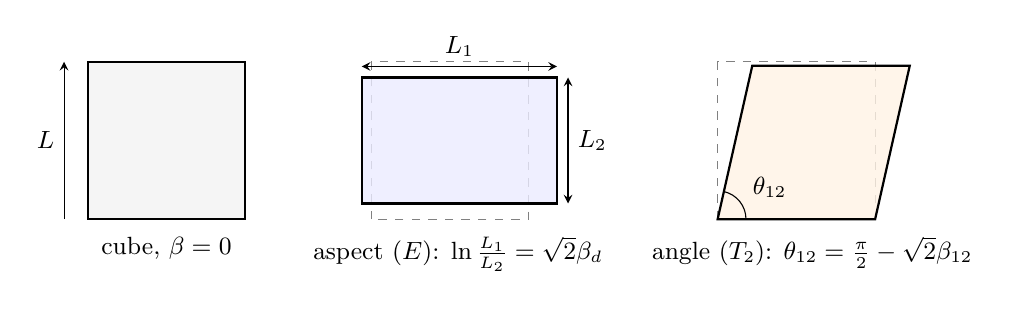
\begin{tikzpicture}[scale=2.0,>=stealth]
  \draw[thick,fill=gray!8] (0,0) rectangle (1,1);
  \node[below] at (0.5,-0.05) {\small cube, $\beta=0$};
  \draw[->] (-0.15,0) -- (-0.15,1) node[midway,left] {\small $L$};
  \begin{scope}[xshift=1.8cm]
    \draw[dashed,gray] (0,0) rectangle (1,1);
    \draw[thick,fill=blue!8,fill opacity=0.8] (-0.06,0.1) rectangle (1.18,0.9);
    \node[below] at (0.55,-0.05) {\small aspect ($E$): $\ln\frac{L_1}{L_2}=\sqrt2\beta_d$};
    \draw[<->] (-0.06,0.97) -- (1.18,0.97) node[midway,above] {\small $L_1$};
    \draw[<->] (1.25,0.1) -- (1.25,0.9) node[midway,right] {\small $L_2$};
  \end{scope}
  \begin{scope}[xshift=4.0cm]
    \draw[dashed,gray] (0,0) rectangle (1,1);
    \draw[thick,fill=orange!10,fill opacity=0.8] (0,0) -- (1,0) -- (1.22,0.975) -- (0.22,0.975) -- cycle;
    \draw (0.18,0) arc (0:77:0.18);
    \node at (0.33,0.2) {\small $\theta_{12}$};
    \node[below] at (0.6,-0.05) {\small angle ($T_2$): $\theta_{12}=\frac\pi2-\sqrt2\beta_{12}$};
  \end{scope}
\end{tikzpicture}
\caption{Shape coordinates of the torus, shown on one face of the fundamental domain at fixed volume.
Left: the cube.
Middle: an aspect deformation along $X_d$, one of the two directions of the representation $E$ of the cubic group; the second, $X_{d2}$, lengthens two edges and shortens the third.
Right: an angle deformation along $X_{12}$, one of the three directions of $T_2$.
Both deformations are drawn far larger than the quantum fossil of Sec.~\ref{rep:quantum-shape}, whose aspect amplitudes are of order $0.1$ and whose angle amplitudes are of order $0.007$.}
\label{fig:rA-shapes}
\end{figure}

\paragraph{Einstein equations.}
For Eq.~\eqref{eq:rA-metric} the flat slices have vanishing intrinsic curvature, and the Gauss--Codazzi relations give the spacetime curvature entirely through $\mathsf K$ (Sec.~\ref{rep:trace}).
The Hamiltonian constraint, $R^{(3)}+\tfrac23\theta^2-\sigma_{ab}\sigma^{ab}=2\rho/\MPbar^2$ with expansion $\theta=3H$ and $R^{(3)}=0$, reads $6H^2-S=2\rho/\MPbar^2$, and Raychaudhuri's equation for the geodesic comoving observers reads $\dot\theta=-\tfrac13\theta^2-S-(\rho+3\bar p)/2\MPbar^2$.
Together
\begin{equation}
3\MPbar^2H^2=\rho+\tfrac12\MPbar^2S,\qquad
\dot H=-\frac{\rho+\bar p}{2\MPbar^2}-\tfrac12S ,
\label{eq:rA-einstein}
\end{equation}
where $\rho$ is the energy density and $\bar p=\tfrac13\Tr p$ the mean pressure; the second equation follows from Raychaudhuri's after eliminating $3H^2$ with the constraint.
The trace-free part of the spatial equations is the shape equation, which the minisuperspace action below gives in a more useful form.

\paragraph{Minisuperspace action.}
Per unit coordinate volume and with unit lapse, the Einstein--Hilbert action of Eq.~\eqref{eq:rA-metric} reduces to $\tfrac12\MPbar^2\sqrt h\,(K_{ij}K^{ij}-K^2)$, with $K_{ij}K^{ij}=\Tr\mathsf K^2=3H^2+S$ and $K=3H$.
Adding matter with energy $E(L,G)=L^3\rho$ gives
\begin{equation}
\mathcal L=-3\MPbar^2L\dot L^2+\tfrac12\MPbar^2L^3\,\tfrac14\Tr\big(G^{-1}\dot G\big)^2-E(L,G),
\label{eq:rA-minisuperspace}
\end{equation}
so the volume has a negative kinetic term and the shape is a sigma model on the space of unimodular metrics, with the metric of Eq.~\eqref{eq:rA-shapemetric} and the inertia $\MPbar^2L^3$.
Variation of the lapse gives the constraint of Eq.~\eqref{eq:rA-einstein}.
Near the cube the shape momenta are
\begin{equation}
P_A=\MPbar^2L^3\dot\beta_A ,
\label{eq:rA-PA}
\end{equation}
and the shape equations are $d(\MPbar^2L^3\dot\beta_A)/dt=-\partial E/\partial\beta_A$ to linear order in $\beta$.
Sections~\ref{rep:gate}, \ref{rep:shape} and~\ref{rep:quantum-shape} use these equations with the Casimir energy as $E$.

\subsection{Units and conventions}
\label{rA:units}

Units are $\hbar=c=1$, and $\MPbar=(8\pi G)^{-1/2}=2.435\times10^{18}$\,GeV is the reduced Planck mass; we never use the non-reduced Planck mass. %
The Planck length is $\ell_{\rm P}=G^{1/2}=1/(\sqrt{8\pi}\,\MPbar)$.
The signature is $(-,+,+,+)$, and the trace of the stress tensor is $T=-\rho+3\bar p$.
We measure time $t$ from the turning point and write $\tau\equiv ht$, where $h$ is the plateau scale of assumption~\ref{assump:A3}; the true rate of the turning-point solution, $\rAHeff=0.98949\,h$, is introduced in Sec.~\ref{rep:turning}. %
In Sec.~\ref{rep:trace} the symbols $a$ and $c$ are anomaly coefficients; elsewhere $a$ is a scale factor.
The couplings $\lambda$, $g_3$, $g_2$, $g_Y$ and $y_t$ are running $\MSbar$ couplings, with $g_Y$ the hypercharge coupling in the Standard Model normalization and the Higgs potential written as $\lambda(\Phi^\dagger\Phi-v^2/2)^2$; unless we say otherwise they are evaluated at the matching scale $\mub$ of assumption~\ref{assump:A2}.
The non-minimal coupling enters the action as $-\xiH R\,\Phi^\dagger\Phi$, so that the conformal value is $\xiH=1/6$.
Quantities in units of $1/L$ are energies of the torus at fixed volume; conformal time $\eta$ is defined by $dt=L\,d\eta$, so that a light ray crosses the torus once per unit of $\eta$.
Notation is collected in Appendix~\ref{rep:app-notation} and the key numbers, with their source files and keys, in Appendix~\ref{rep:app-numbers}.

\subsection{Field contents}
\label{rA:content}

Two field contents recur.
The \emph{Standard Model} content is its high-energy field content, the twelve gauge vectors, the Higgs doublet and 45 Weyl fermions (no right-handed neutrinos), together with the static graviton, whose two polarizations count as one Maxwell field in the Casimir energy. %
In units of the Casimir energy of one Maxwell field, which has two physical polarizations, the bosons count $B=12+2+1=15$: twelve vectors, the four real Higgs components (two units) and the graviton.
The fermions count $F=45$, one unit per Weyl fermion.
The \emph{Maxwell toy} consists of $N_v$ periodic Maxwell fields plus the static graviton; it is a controlled model for which we also compute the causal response and the nonlinear evolution of the shape (Secs.~\ref{rep:shape} and~\ref{rep:quantum-shape}).

\subsection{Assumptions}
\label{rA:assumptions}

Our results rest on eight assumptions, which we state here once.
\begin{itemize}
\item[(A1)]\rAassume{assump:A1}
Einstein gravity sourced by the expectation value of the stress tensor, $\MPbar^2G_{\mu\nu}=\langle T_{\mu\nu}\rangle$, for homogeneous expectation values~\cite{Hartle:1981zt}, with the volume and the inflaton treated classically, except where Secs.~\ref{rep:quantum-shape} and~\ref{rep:sky} quantize the volume and the inflaton zero mode to test the reality condition, the shear criterion and the spread of sizes, and with the shape moduli and the zero modes treated quantum mechanically.
Space is a flat three-torus; the fermions are antiperiodic around all three cycles (the AAA spin structure), the gauge holonomies are trivial, and there is no 't~Hooft flux.
\item[(A2)]\rAassume{assump:A2}
The Standard Model, with a non-minimal coupling $\xiH R\,\Phi^\dagger\Phi$ of the Higgs doublet to the Ricci scalar, holds up to the scale $2\pi\mub$ of the lowest non-zero modes, where $\mub\equiv1/\Lb=\MPbar/722\simeq3.4\times10^{15}$\,GeV is the matching scale. %
Its $\MSbar$ couplings at $\mub$ follow from next-to-next-to-leading-order (NNLO) matching at the top-quark mass and three-loop running, with $M_h=125.13$\,GeV and $\alpha_s(M_Z)=0.1180$~\cite{ParticleDataGroup:2026mpi} (Sec.~\ref{rep:h-smmap}). %
New states below $\mub$ that couple to the Higgs would change $\lambda(\mub)$: Yukawa couplings of heavy right-handed neutrinos lower it~\cite{Casas:1999cd,Rodejohann:2012px} and would move the criterion of Sec.~\ref{rep:h-smmap} to smaller $\mt$, whereas extra scalars can raise it; the criterion tests the Standard Model up to $2\pi\mub$.
Heavier states that couple to the Higgs field would generate a term $c\,\phi^6/M^2$ with $M<\MPbar$, and the criterion assumes that such states, if present, lie near $\MPbar$ or couple weakly to the Higgs field (Sec.~\ref{sec:v11-mechanism-context}).
\item[(A3)]\rAassume{assump:A3}
An inflaton with a plateau potential supplies the negative trace at the turning point (Sec.~\ref{rep:trace}) and the inflation that follows.
Our benchmark member of this family is
\begin{equation}
V(\phi)=3\MPbar^2h^2\big(1-e^{-\sqrt{2/3}\,\phi/\MPbar}\big)^2,
\label{eq:rA-plateau}
\end{equation}
the Einstein-frame potential of Starobinsky's model~\cite{Starobinsky:1980te} for a minimally coupled scalar, with $h$ fixed by the observed scalar amplitude (Sec.~\ref{rep:turning}), and the error budget of Sec.~\ref{rep:h-budget} varies the inflation scale over the family.
The inflaton enters the Higgs results only through $\mub$ and the duration of the turn: we assume no direct inflaton--Higgs coupling (portal or mixed non-minimal terms).
\item[(A4)]\rAassume{assump:A4}
The turning point is a beginning: each of the two branches, the contracting one before the turn and the expanding one after it, is read with its arrow of time pointing away from the turn (Sec.~\ref{rep:gate}).
$\Pone$ is the survival probability of the Higgs zero mode along one branch, conditional on its being in the finite-volume resonance at the turn.
The preparation weight of that resonance, $w_0=0.98$--$0.995$, follows from the rule of assumption~\ref{assump:A8}, the time-symmetric Gaussian of minimal energy variance (Sec.~\ref{rA:s-equivalent}), applied to the Higgs zero mode (Sec.~\ref{rep:h-survival}). %
\item[(A5)]\rAassume{assump:A5}
The dynamics of the Higgs zero mode is computed in the reduced model of Sec.~\ref{rep:h-reduced}, whose errors, including a full-dimensional check (Sec.~\ref{rep:v-fulldim}), are collected in the error budget of Sec.~\ref{rep:h-budget}.
\item[(A6)]\rAassume{assump:A6}
$\xiH$ is defined at $\mub$: it is the coefficient of $R\,\Phi^\dagger\Phi$ in the zero-mode Hamiltonian at the turn, and its electroweak-scale image follows from its running (Sec.~\ref{rep:h-universality}).
\item[(A7)]\rAassume{assump:A7}
$\mt$ denotes the top-quark pole mass, obtained from the $\MSbar$ mass with the pole--$\MSbar$ relation truncated at four loops, and $\mtbar\equiv\mtbar(\mtbar)$ is the $\MSbar$ mass.
We identify the direct (Monte Carlo) mass, $172.60\pm0.27$\,GeV~\cite{ParticleDataGroup:2026mpi}, with $\mt$ up to an interpretation uncertainty of about $0.5$\,GeV~\cite{Hoang:2020iah}, and use the MSR mass as a variant (Sec.~\ref{rep:h-smmap}). %
\item[(A8)]\rAassume{assump:A8}
At the turn the shape moduli are in the natural state: the time-symmetric Gaussian of minimal energy variance, centered on the cube (Secs.~\ref{rA:s-floor} and~\ref{rA:s-equivalent}), whose outgoing variance lies $0.05\%$ above the floor of Sec.~\ref{rA:s-floor}. %
The fossil and sky predictions of Secs.~\ref{rA:s-fossil} and~\ref{rep:sky} refer to this state; Sec.~\ref{rep:quantum-shape} also treats other states.
\end{itemize}
Section~\ref{rep:trace} needs only \ref{assump:A1} and the hypotheses stated with its obstruction, Secs.~\ref{rep:casimir}--\ref{rep:turning} add \ref{assump:A2} and \ref{assump:A3}, \ref{assump:A4}--\ref{assump:A7} enter from Sec.~\ref{rep:h-matching} on, and \ref{assump:A8} enters in Secs.~\ref{rep:quantum-shape} and~\ref{rep:sky}.
The emptiness gate of Sec.~\ref{rep:gate} motivates \ref{assump:A4}; the gate allows the vacuum states that \ref{assump:A4} and \ref{assump:A8} specify but does not enforce them.
Later chapters refer to these assumptions by number and do not repeat them.

\subsection{Scope of the free-field description}
\label{rA:scope}

Within this setup the Casimir energy is that of the nonzero modes of free massless fields with flat twists; their interactions enter through the one-loop finite-volume potential of the zero modes (Sec.~\ref{rep:zeromodes} and Sec.~\ref{rep:h-matching}).
All Standard Model masses are negligible at the turn, where $1/\Lb$ exceeds the electroweak scale by thirteen orders of magnitude, $\mub/v=3.37\times10^{15}/246\simeq1.4\times10^{13}$. %
Perturbative interactions of the nonzero modes correct the Casimir weights by a relative amount of order $g^2/16\pi^2$ (Sec.~\ref{rep:casimir}).
The shape moduli are treated as collective coordinates of the geometry, with the Casimir energy as their potential; the response of the fields to a moving shape is a correction of relative order $10^{-6}$ (Sec.~\ref{rep:shape}).

\subsection{Status of results and numbers}
\label{rA:status}

We label every result by the kind of evidence behind it.
A result is \emph{proved} when it follows from the stated equations by an argument given in full, \emph{conditional} when it holds under a stated hypothesis of the model or of the setting, \emph{numerically tested} when it rests on computations with documented convergence and independent checks, and \emph{open} otherwise.
Theorems and propositions are proved statements within the stated model; survival thresholds and probabilities are numerical.
Numbers that enter the claims of the companion papers are typeset with the macros of the shared files \texttt{numbers.tex} and, for the static box and the abelian Higgs model, \texttt{numbers\_c170.tex}; every other number carries, at the end of its source line, a tag \texttt{\%~[num:...]} that names its entry in the number inventories or its source file and key.
Superseded values and abandoned approaches are collected in Part~III (Sec.~\ref{rep:history}) and are not used in Part~I.
